\chapter{Literature review}
\label{chap-two}
Bridges are designed based on discrete events assuming that the initial material and structure properties remain constant through the life of the bridge. The purpose of the research described is to study condition dependent performance based design that considers the material and geometric properties as the structure ages, and the effects of multiple and discrete events on the achievement of prescribed limit states.

In this chapter, the current knowledge of aging of structures, damage indexes, corrosion and multiple earthquake loading is presented. Then the study gap and the objectives of this research are defined.

\section{Corrosion}

Corrosion is one of the main aging effects in RC structures.In RC structures after the concrete is cast a protective layer forms on the surface of the reinforcing steel, this process is known as passivation of the reinforcing steel. However, under conditions such as chloride attack the protective film is can be broken, this process is known as depassivation.The depassivation process onsets corrosion. Corrosion reduces the area of steel, and also modify the strength of the reinforcing steel. If corrosion degrades the structural performance of the reinforcing steel it will certainly degrade the overall strength of the system. The incidence of corrosion in RC structures in earthquake prone areas is that it could trigger unintended seismic performance on a structure that was designed for pristine conditions. Therefore it is important to incorporate the  mechanics of corrosion in this condition dependent performance based seismic design. The general chloride attack corrosion process can be explained using three main parameters such as (1) time to initiation of corrosion, (2) corrosion growth in reinforcing steel, and (3) the mechanical properties of corroded reinforcing steel. Figure \ref{fig:corr1} schematically shows the corrosion process.

\begin{figure}[htbp]
\centering
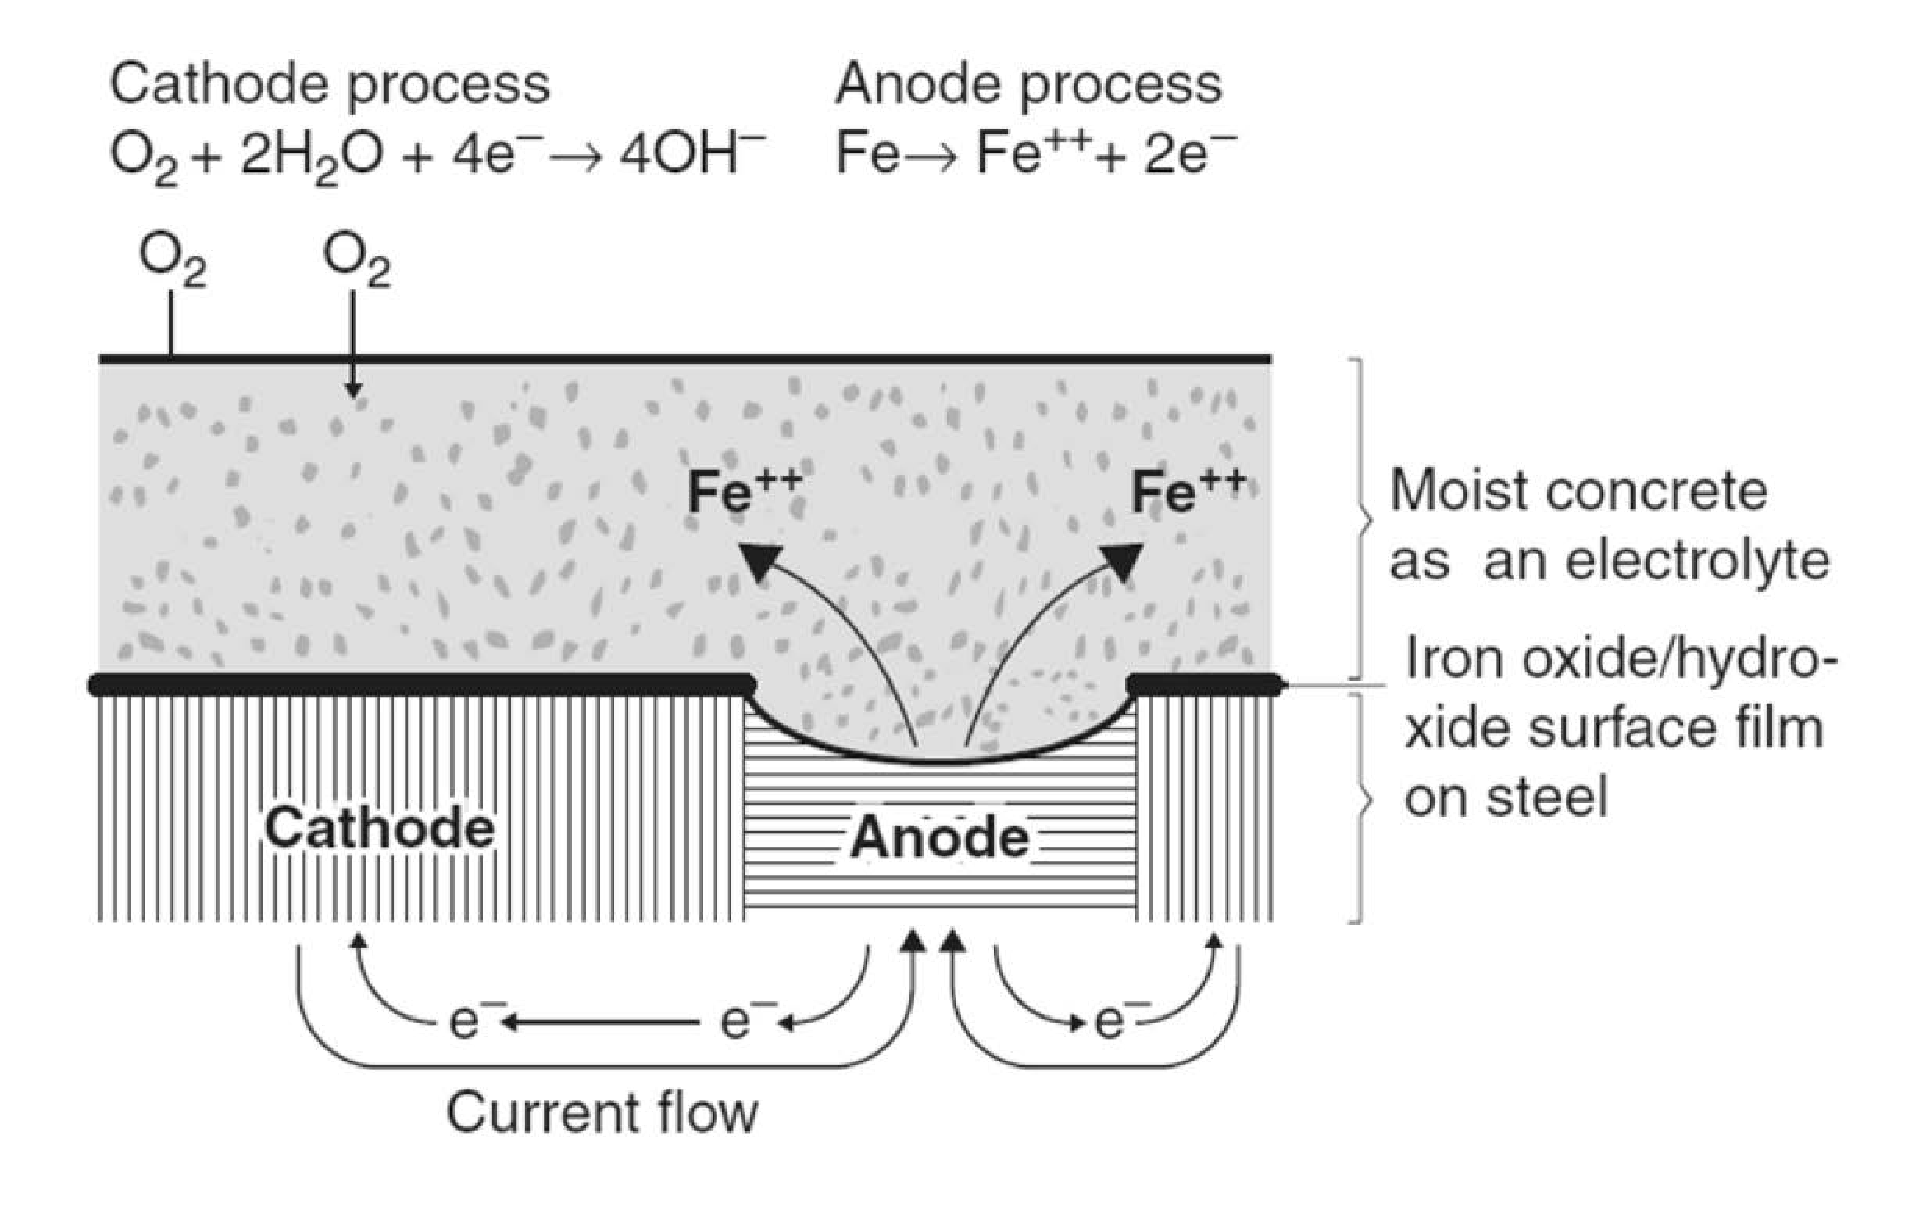
\includegraphics[width=0.9\textwidth]{Chapter-2/figs/Corrosion_Process}
\caption{Corrosion process in reinforcing steel bar \cite{Mehta2014}}
\label{fig:corr1}
\end{figure}

\subsection{Time to corrosion}

 Jensen et al performed a series of experiments to measure the chloride ingress in the cement and mortar paste  \cite{Jensen1999}. In their study, it was determined that the ingress of chlorides follows Fick's law of diffusion, shown in \eref{eq:ficks_law}. Stewart et al solved \eref{eq:ficks_law}  in terms of the chloride ion concentration ($C(x,t)$), distance from concrete surface ($x$), time of exposure to chloride ions ($t$), and the chloride diffusion coefficient ($D_c$). The solution rendered equation \eref{eq.three} which describes the time to initiation of corrosion    \cite{Stewart1998}\cite{Y.Liu1998a}\cite{Thoft-Christensen}. Mean values for $C_0$ and $C_r$ have been previously defined for environments that are controlled by deicing salts \cite{Ghosh2010}\cite{Weyers1994}\cite{Enright1998}.

\begin{equation}
	\frac{\partial C(x,t)}{\partial t} = D_c \frac{\partial C(x,t)}{\partial x^2}
	\label{eq:ficks_law}
\end{equation}
\newline
\begin{equation}
  T_{corr}=\frac{x^2}{4 D_c} \left[erf^{-1} \left(\frac{C_0-C_{cr}}{C_0} \right) \right]^{-2}
  \label{eq.three}
\end{equation} 

\subsection{Rate of corrosion}

Vu et al developed an empirical model to evaluate the corrosion rate \cite{Vu2000}\cite{Stewart1998}. In their study a constant corrosion rate was assumed. However, it is known that the corrosion rate is not constant over time because it is dependent on factors such as the quality of concrete, the amount of oxygen available in the environment, and the relative humidity.  Nonetheless, for long term studies this approximation is valid. The underlying assumptions of this model are a relative humidity of 75\% and a temperature of 20°C. The model developed by Vu et al is shown in \eref{eq.CorrosionRate}. Figure \ref{fig:hist1} shows the corrosion rate for different concrete covers ($d_c$), as a function of the water to cement ratio ($w/c$). In general, for large values of cover depth the rate of corrosion decreases rapidly, and as the water to cement ratio (i.e. lower quality concrete) increases the rate of corrosion increases.

\begin{equation}
  i_{corr}=\frac{37.5(1-w/c)}{d_c}
  \label{eq.CorrosionRate}
\end{equation} 

\begin{figure}[htbp]
\centering
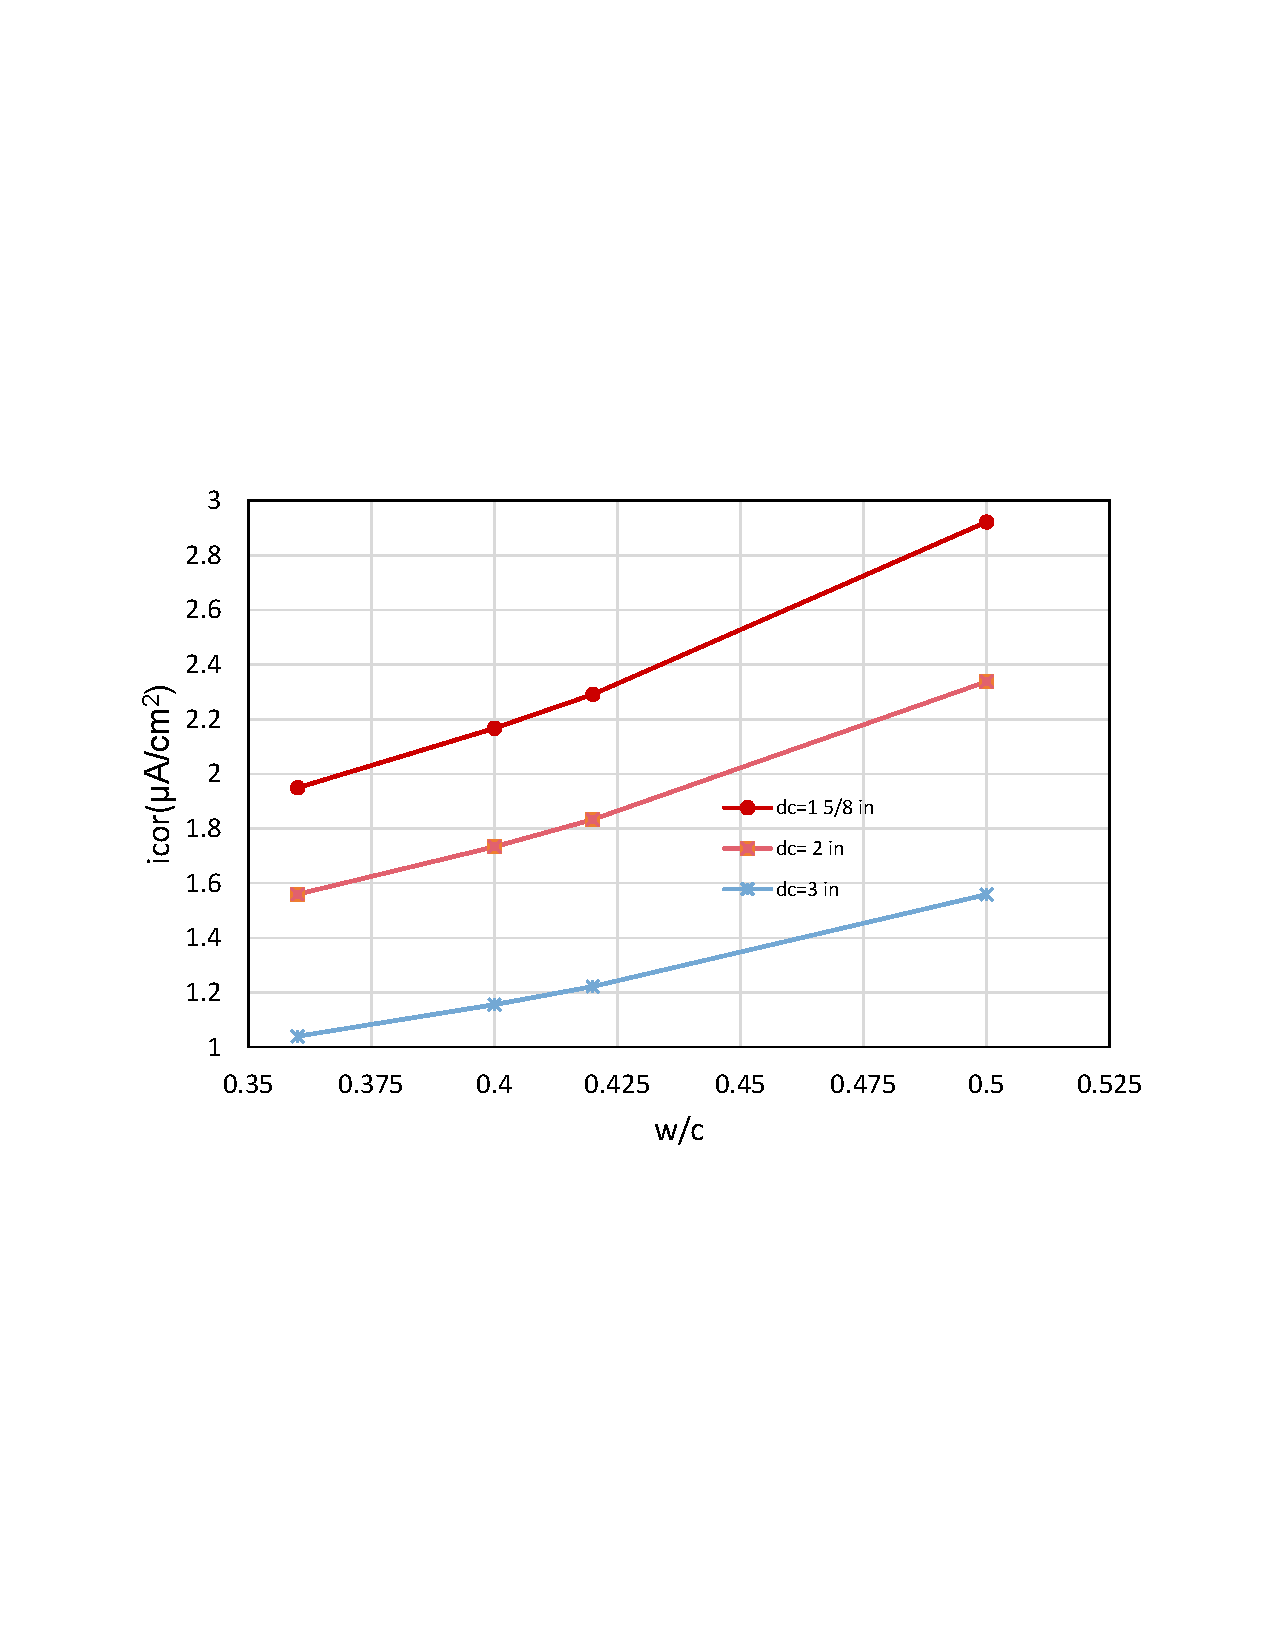
\includegraphics[width=0.85\textwidth]{Chapter-2/figs/wc_icor}
\caption{Concrete water to cement ratio vs rate of corrosion}
\label{fig:hist1}
\end{figure}

In addition, Vu et al  further improved the model of corrosion growth in reinforcing steel developed by Stewart et al \cite{Vu2000}\cite{Stewart1998}\cite{Choe2008}\cite{Ghosh2010}. Their proposed model describes the reduction in diameter of reinforcing steel ($d_{corr}(t)$ as a function of time described in \eref{eq.CorrosionEvolution}. Figure \ref{fig:DiameterEvolution} shows this model applied to a rebar with an initial diameter ($d_{bi}$) of 3/4 inch, a concrete cover of 1-1/2”, and water to cement ratios ranging from 0.36-0.50.

\begin{equation}
  d_{corr}(t)=d_{bi}-\frac{1.0508(1-w/c)}{d_c} (t-t_{corr})^{0.71}
  \label{eq.CorrosionEvolution}
\end{equation} 

\begin{figure}[htbp]
\centering
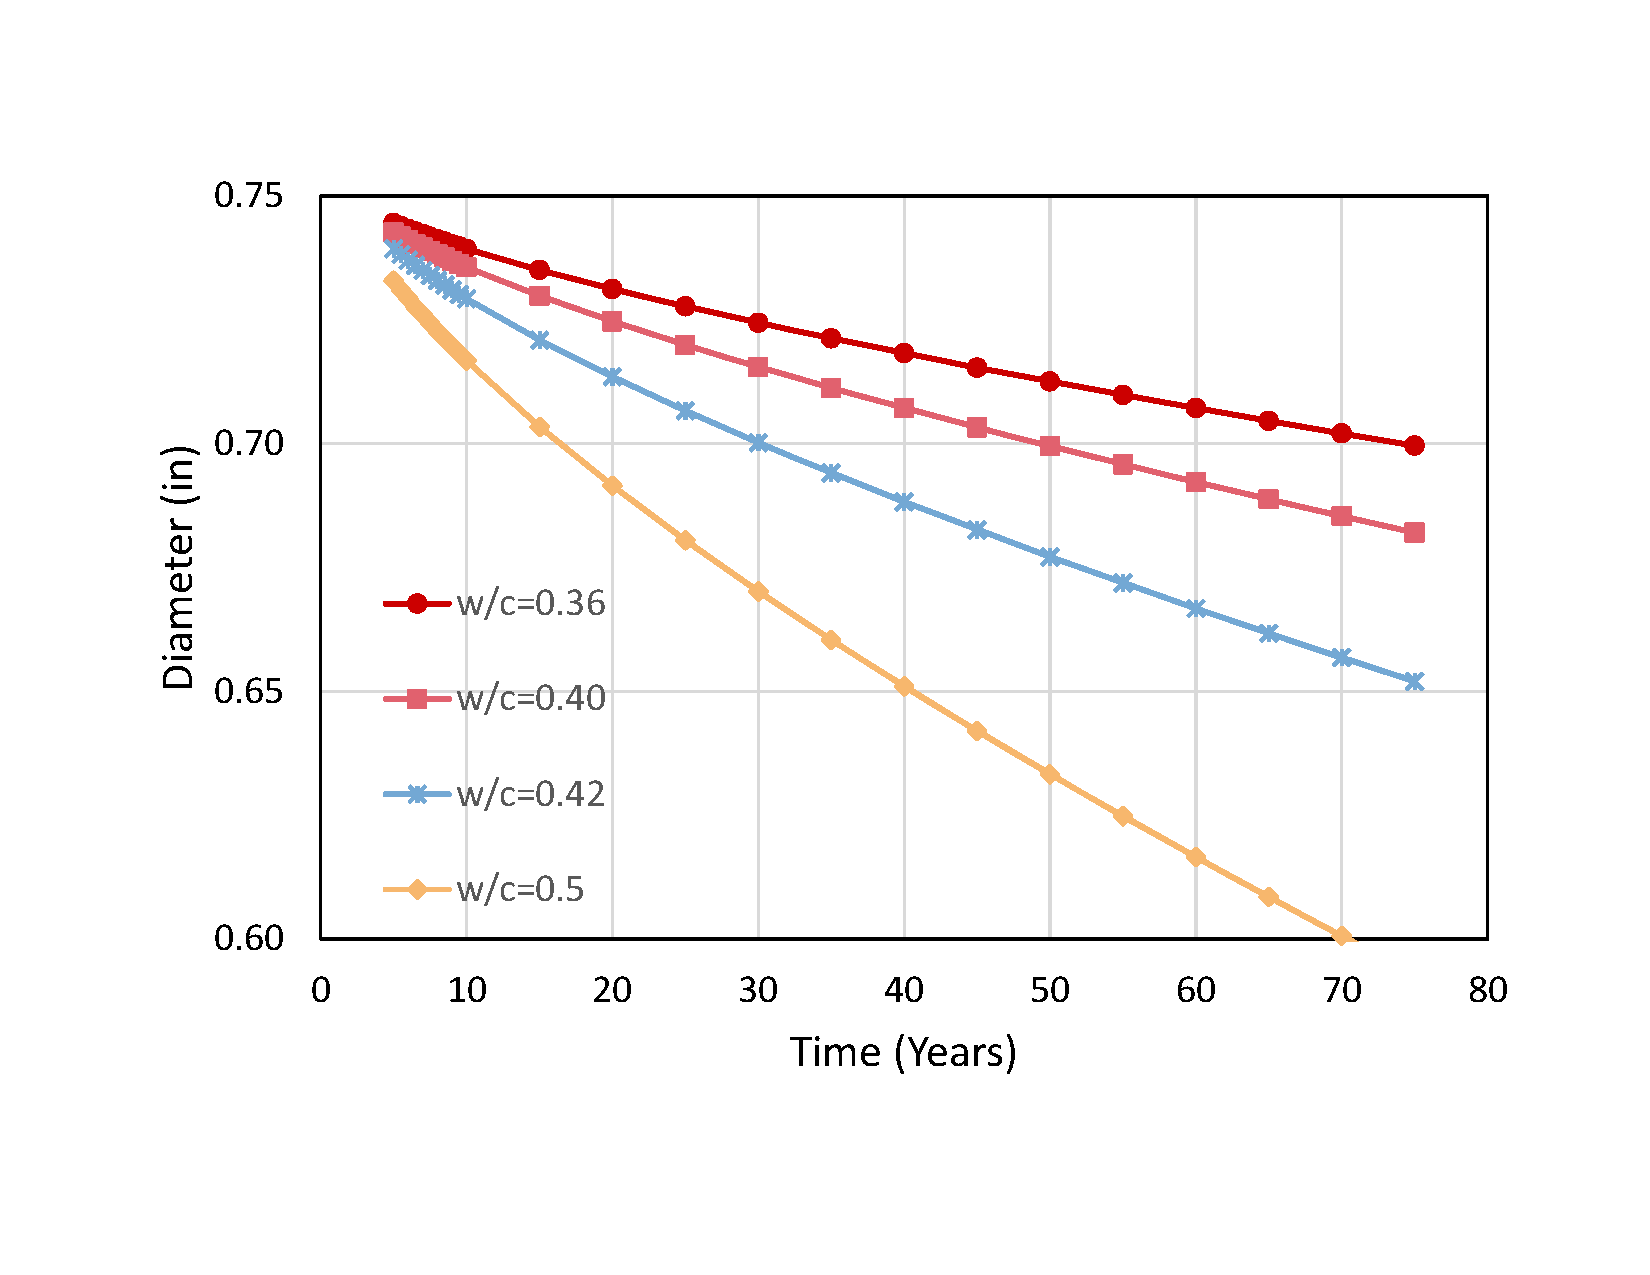
\includegraphics[width=0.85\textwidth]{Chapter-2/figs/DiameterDecrease}
\caption{Diameter decrease due to corrosion}
\label{fig:DiameterEvolution}
\end{figure}

Further, the evolution of corrosion in reinforcing steel can be expressed in the percent loss of mass of a rebar. If uniform corrosion is assumed, this can be expressed as the percent of reduction of diameter. The corrosion level can be expressed as shown in \eref{eq.CorrosionLevel}.

\begin{equation}
	CL=\frac{d_{bi}-d_{corr}(t)}{d_{bi}}*100%
  \label{eq.CorrosionLevel}
\end{equation} 

Combining \eref{eq.CorrosionEvolution} with \eref{eq.CorrosionLevel},  the variation of the corrosion level can be described as a function of time. Figure  \ref{fig:CorrosionLevel_Time} shows the results of this process.

\begin{figure}[htbp]
\centering
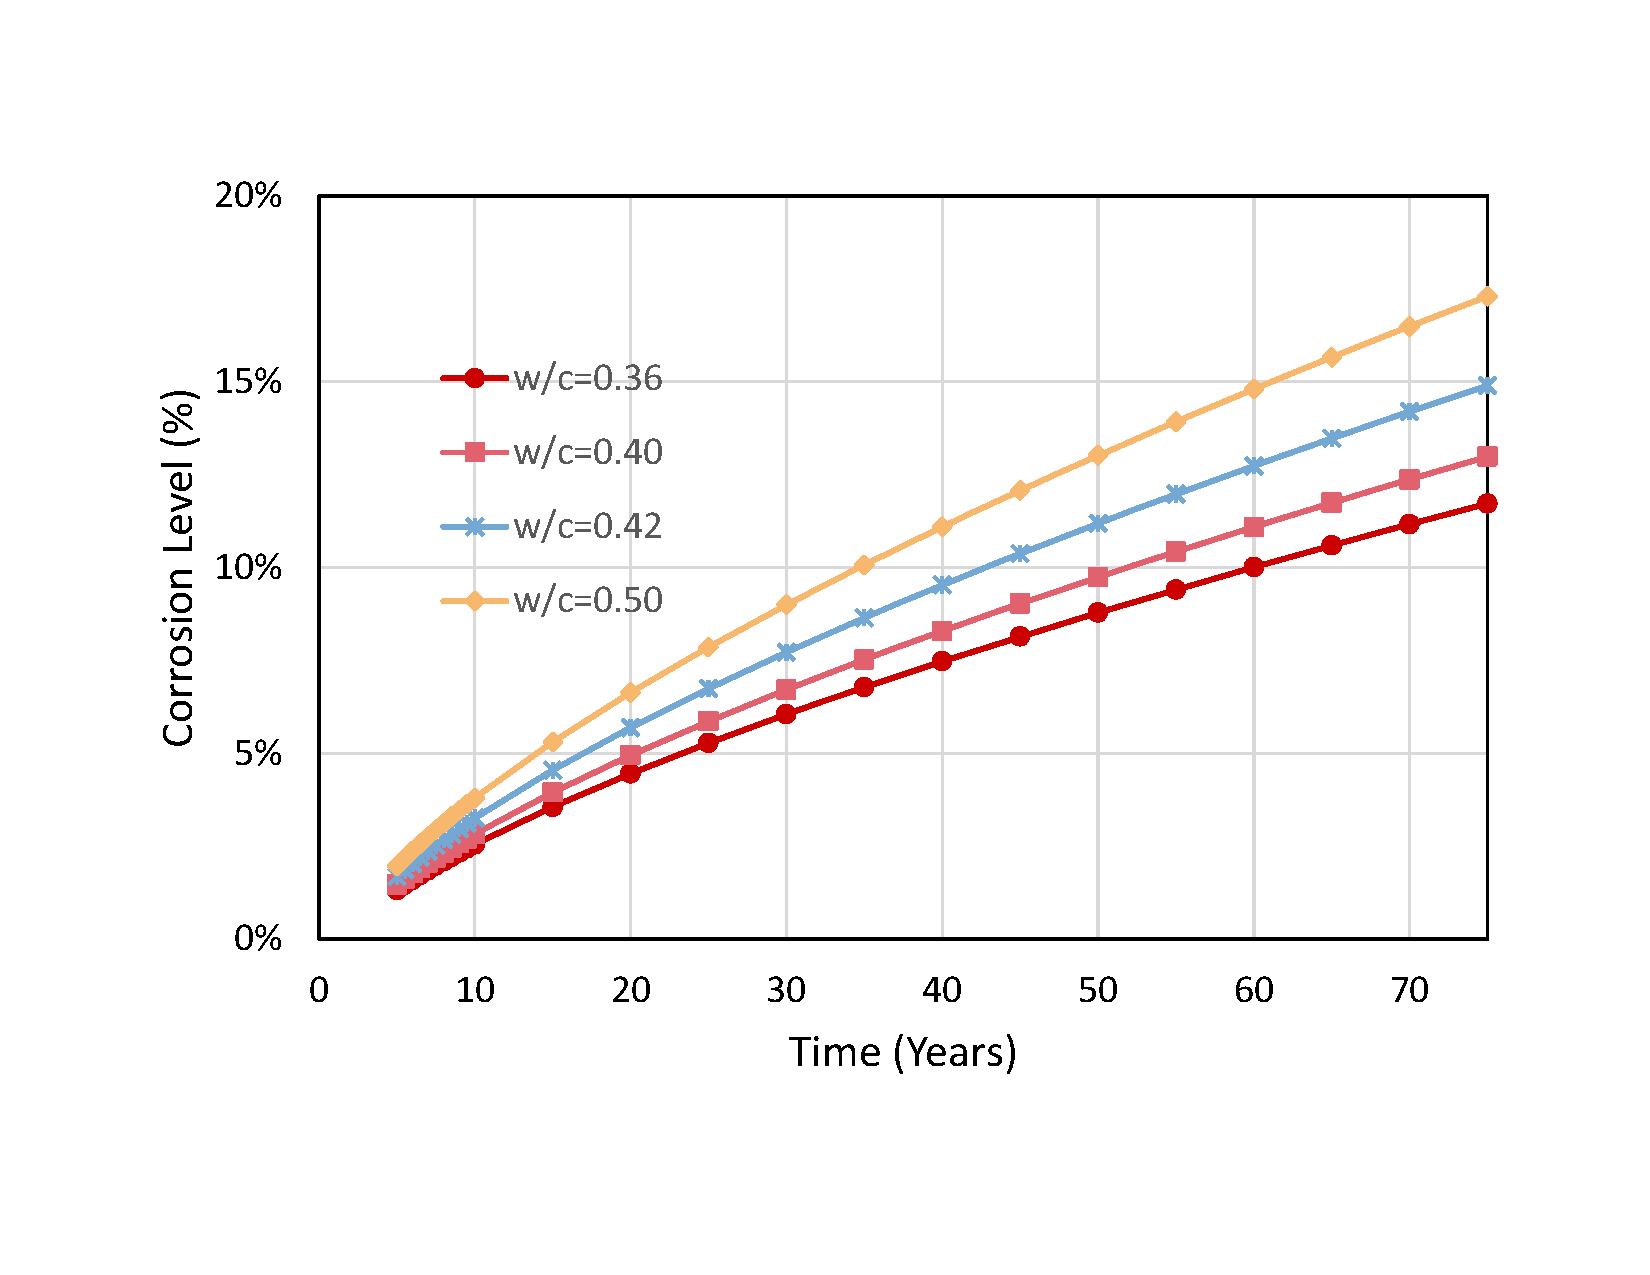
\includegraphics[width=0.85\textwidth]{Chapter-2/figs/CorrosionLevel}
\caption{Corrosion level vs time (years)}
\label{fig:CorrosionLevel_Time}
\end{figure}

\subsection{Corrosion modified properties of reinforcing steel bars}

Yuan et al \cite{Yuan2017a} performed tension tests on corroded rebars and determined that the mechanical properties of steel change with the level of corrosion. In general, as corrosion increases, the yield strength and ultimate strength of the reinforcing steel decrease.  The variation of the mechanical properties is shown in \eref{eq.eleven} for the yield strength and ultimate strength of the reinforcing steel.

\begin{equation}
  f_{y,CL}=f_{yo}(1-0.021CL)
  \label{eq.eleven}
\end{equation} 
\[
  f_{u,CL}=f_{uo}(1.018-0.019CL)
\]

One of the limitations in their study is that the accelerated corrosion process used to develop the corrosion in the rebars did not account for the depassivation process that naturally occurs in rebars embedded in concrete. Chapter \ref{chap-three} shows a proposed experimental assessment that will provide an accurate evaluation of the mechanical properties of corroded reinforcing steel. 

\subsection{Physical test on corroded RC Structures}

Recent studies \cite{Ma2012}, \cite{Meda2014} and \cite{Yang2016} have been developed to assess the effect of corrosion in the structural performance of cantilever RC columns. These columns were were subjected to accelerated corrosion to obtain different corrosion levels ($CL$). The range of $CL$ for these studies correspond to $CL=0\%-20\%$. In these studies the accelerated corrosion was performed via an electrochemical process directly applied to the reinforcing steel as shown in \fref{fig:Meda_RC_CorrosionProc}.

\begin{figure}[htbp]
	\centering
	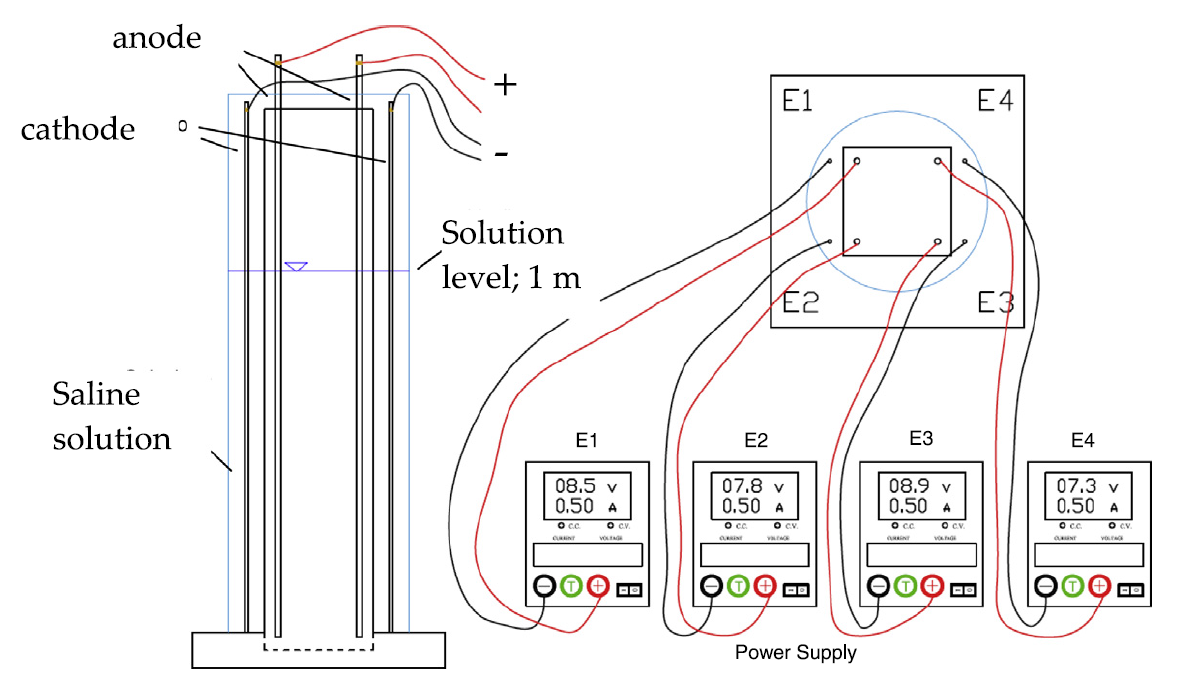
\includegraphics[width=0.7\textwidth]{Chapter-3/figs/Meda_Corrosion}
	\caption{Force displacement response of RC corroded columns \cite{Meda2014}}
	\label{fig:Meda_RC_CorrosionProc}
\end{figure}

The corroded RC columns where then subjected to a quasi-static loading protocol. The resulting force displacement response of one of these experiments is shown in \fref{fig:Meda_FD}. It can be seen that there is a reduction of he strength and displacement capacity of the system. 

\begin{figure}[htbp]
	\centering
	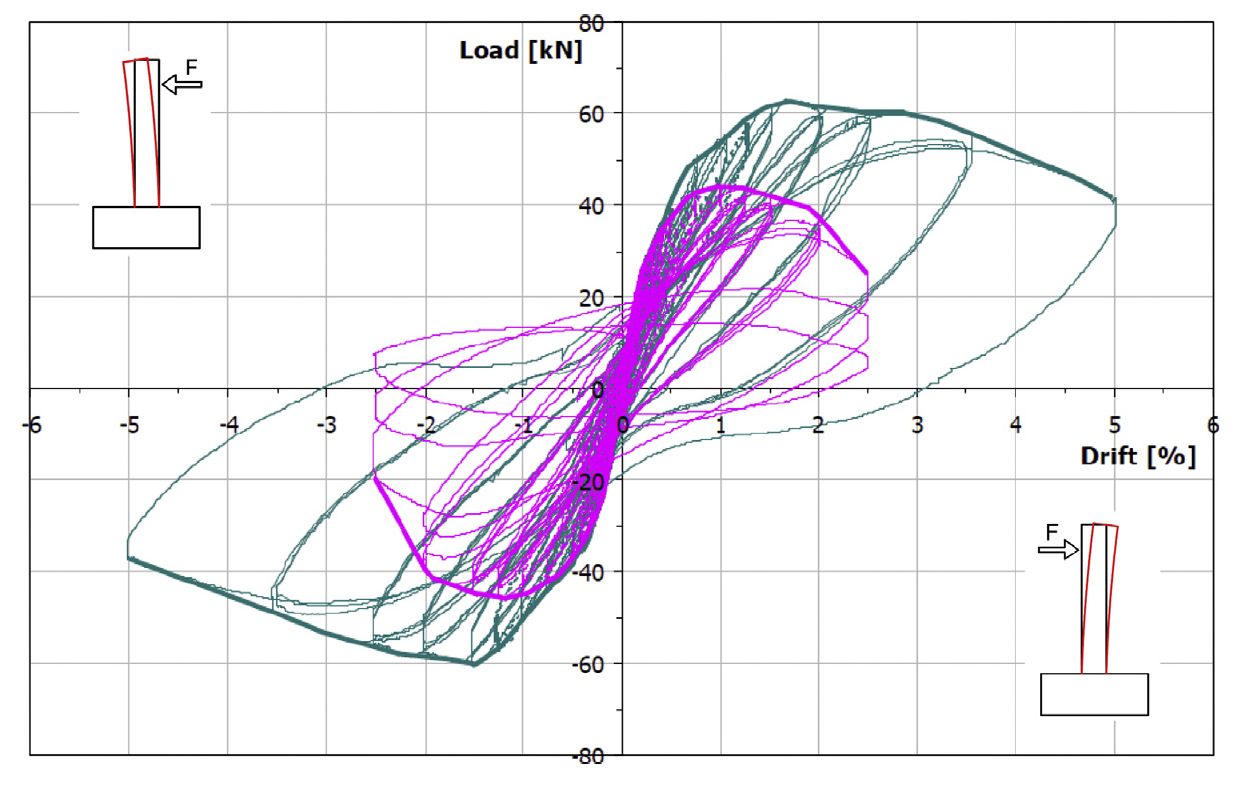
\includegraphics[width=0.7\textwidth]{Chapter-3/figs/Meda_F-D_01}
	\caption{Corrosion process for RC column \cite{Meda2014}}
	\label{fig:Meda_FD}
\end{figure}

As stated in the previous section the mechanical properties of steel are affected by corrosion. In the previous studies \cite{Meda2014} the authors performed tension tests on corroded reinforcing steel. In these tests a reduction in the mechanical properties of steel was observed as well as a reduction in the rupture strain $\varepsilon_{srup}$, see \fref{fig:Meda_RebarTest}. 

\begin{figure}[htbp]
	\centering
	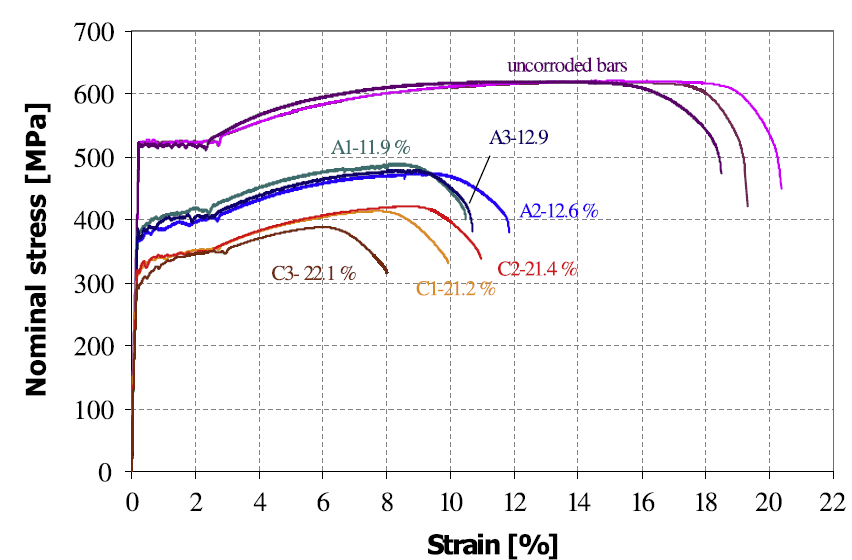
\includegraphics[width=0.7\textwidth]{Chapter-3/figs/Meda_StressStrain}
	\caption{Corroded rebars stress-strain curves \cite{Meda2014}}
	\label{fig:Meda_RebarTest}
\end{figure}

While these studies show how corroded RC columns behave under cyclic loading, they did not consider the generation of the protective film due to the alkaline environment of the concrete. This film can modify the mechanical properties of corroded steel. In addition, the accelerated corrosion process used a 3\% $NaCl$ concentration solution while the chloride attack in concrete usually has a 1.0\% - 1.5\% concentration of the same chloride. Therefore the results obtained from these studies do not accurately represent the actual conditions of corroded RC columns. Thus, an experimental campaign is proposed that will provide results on the mechanical behavior of corroded reinforcing steel inside concrete. The experimental campaign is discussed in Chapter \ref{chap-three}.

\section{Steel strain aging}

While corrosion is an important parameter that affects steel in structures, strain aging is a phenomenon that affects mild steels, which are common in older structures. Strain aging is the process in which steel after being subjected to large strains and an amount of time passes after the loading, when the steel is reloaded it presents a higher strength and reduced ductility than before the first loading. Therefore the incorporation of this parameter in this research will help evaluate this effect in older structures when subjected to repeated earthquake loading. This process is explained in more detail in this section.

\subsection{Metallurgical process}

It is generally accepted that strain aging is due to the diffusion of carbon and/or nitrogen atoms in solution to dislocations that have been generated by plastic deformation. Initially, an atmosphere of carbon and nitrogen atoms is formed along the length of a dislocation, immobilizing it. Extended aging, however, results in sufficient carbon and nitrogen atoms for precipitates to form along the length of the dislocation\cite{Overby2017}\cite{Hosseini2015}.

These precipitates impede the motion of subsequent dislocations and result in some hardening and loss in ductility. The extent of strain aging, which is a thermally activated process, depends primarily on aging time and temperature. In general, extended aging results in a saturation value above which further aging has no effect \cite{Restrepo-Posada1994}.

A second strengthening mechanism occurs when cold deformation (alone) is applied to steels. When dislocations break away from their pinning interstitial atoms and begin the movement causing slip they begin to intersect with each other. A complex series of interactions between the dislocations occurs, causing them to pin each other, decreasing their mobility. The decreased mobility also results in higher strength, lower ductility and lower toughness. As a result, cold deformed steels already have lowered ductility and toughness before any strain aging occurs. When heating follows cold deformation, the loss in ductility and toughness is greater. It is this combination of events that is the most damaging to the toughness of structural steels \cite{Momtahan2009}.

\subsection{Strain aging effects in structures}

Strain aging is the process by which steel after being subjected to large strains, develops an increased strength and reduced ductility with time. Large earthquakes can cause this effect on structures built with mild steel. Therefore, it is  important to include strain aging in a time dependent analysis. Furthermore, strain aging will cause an increase in the strength of the plastic hinge and as a consequence plastic hinges may form in regions of the structures that have not been designed for such demands. The effects of strain aging may also alter the transverse reinforcement due to cold bending, making them susceptible to brittle failure\cite{Momtahan2009}.

According to Restrepo-Posada\cite{Restrepo-Posada1994}, most strain aging occurs in the first 37 days. In addition, Momtahan et al  \cite{Momtahan2009} studied strain aging effects with respect to time at different levels of pre-strains. The pre-strains ranged from $2\varepsilon_y $ to $10\varepsilon_y$, for a time frame of 3 days to 50 days. Their results determined that a significant effect of strain aging took place from pre-strains $5\varepsilon_y$ and on. Strains higher than $15\varepsilon_y$ indicate a performance level in which substantial damage has been induced in the structure such that it is deemed unrepairable and therefore pre-strains higher that $15\varepsilon_y$ are impractical and were not studied \cite{Momtahan2009}.

Momtahan et al correlated the increase in yield strength as a function of time and the pre-strain in reinforcing steel bars. The proposed equations are shown below:

For $10\varepsilon_y$

\begin{equation}
  \frac{f_y}{f_{yi}}=0.0026t+0.9838
  \label{eq.twelve}
\end{equation} 

For $5\varepsilon_y$

\begin{equation}
  \frac{f_y}{f_{yi}}=0.0008t+0.996
  \label{eq.thirteen}
\end{equation} 

For $2\varepsilon_y$

\begin{equation}
  \frac{f_y}{f_{yi}}=0.0004t+0.9979
  \label{eq.fourteen}
\end{equation} 

It is proposed to limit the increase in yield strength obtained at 50 days, which was the limit of scope of their study. Equations \ref{eq.twelve} to  \ref{eq.fourteen} are plotted in \fref{fig:hist4}

\begin{figure}[htbp]
\centering
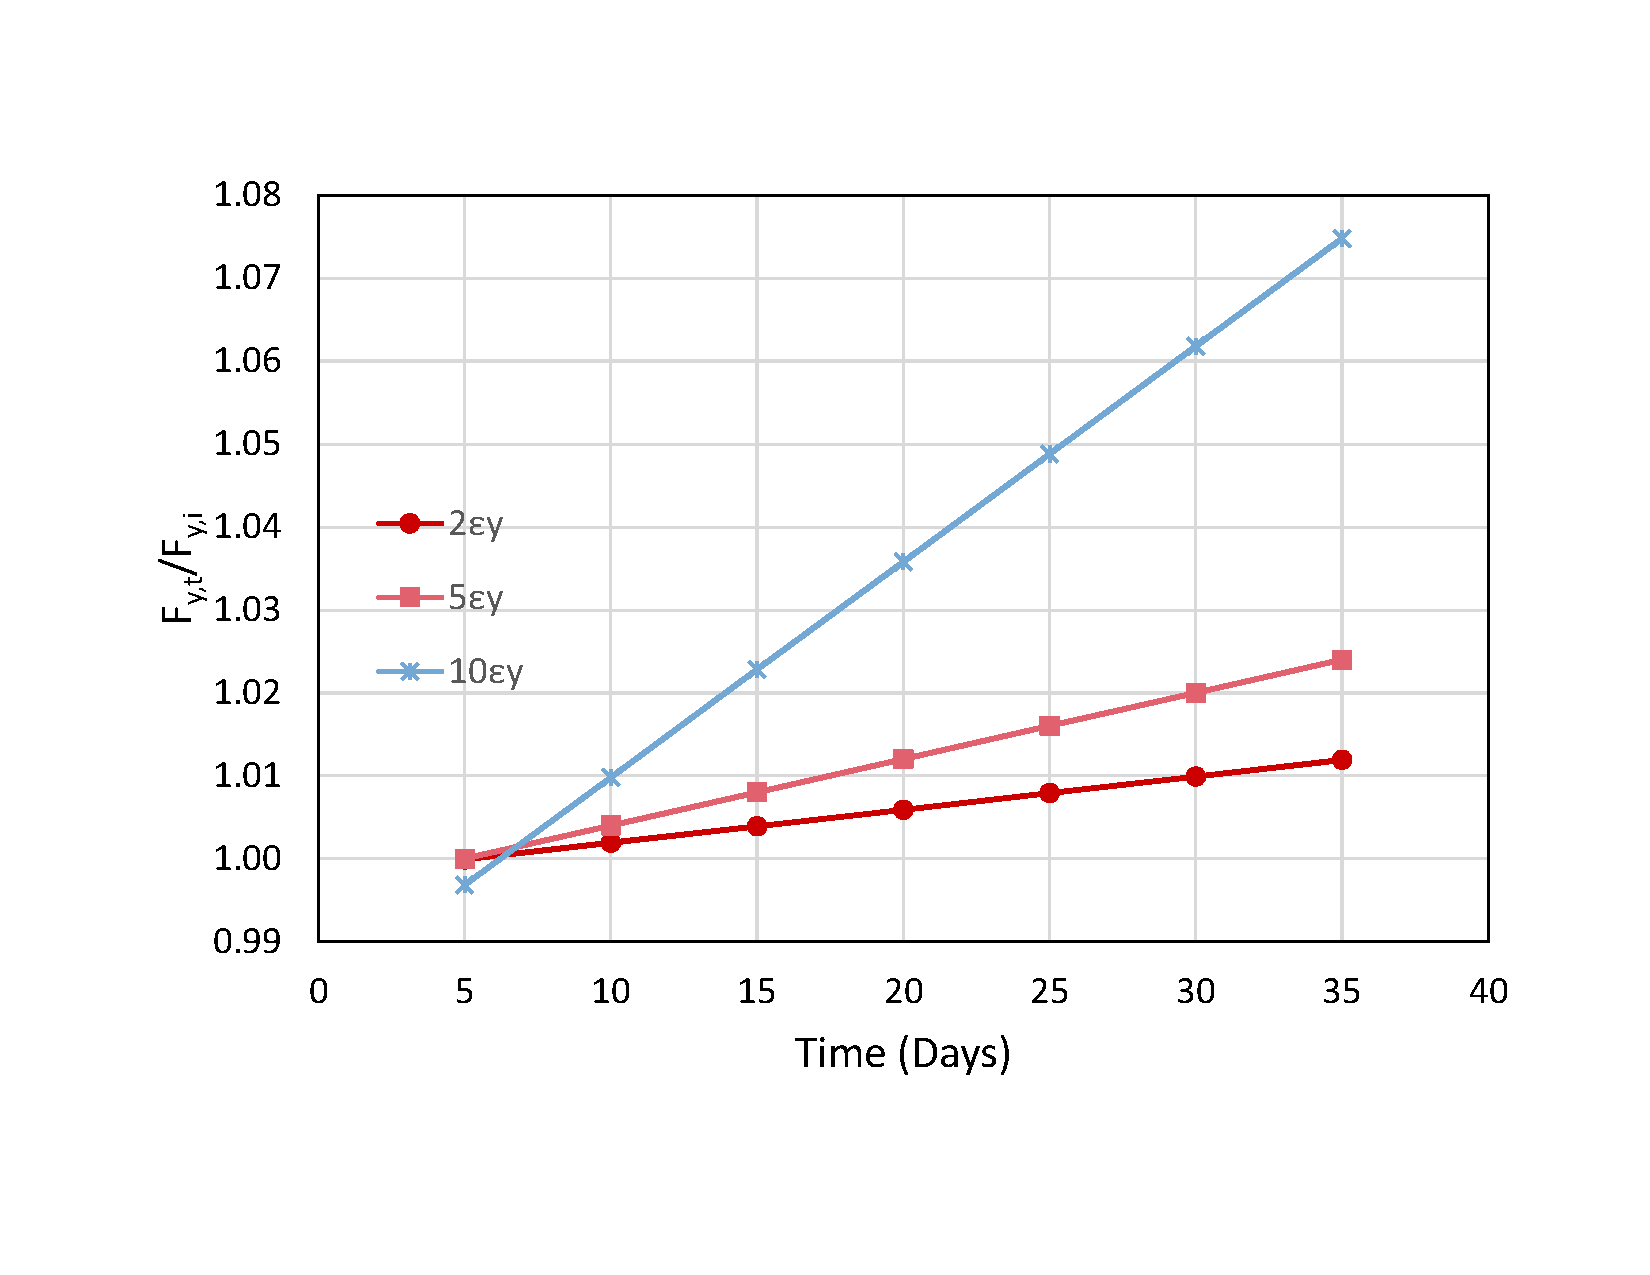
\includegraphics[width=0.7\textwidth]{Chapter-2/figs/StrainAging_TimeDependent}
\caption{Strain aging effect on yield strength vs time (days)}
\label{fig:hist4}
\end{figure}

\newpage

\section{Damage Indexes}
The use of damage indexes has dominated the research related to damage accumulation. While these methods are practical and appear to have a logical basis, they are based on empirical relationships and need to be correlated for each structure case to be of any significance. An example is shown in this section demonstrate this inconsistency.  The literature review presented here is to understand what has been done previously to study the effect of damage accumulation, however it is the purpose of this research that strain limit states are an improved measure of damage over empirical methods.

The effect of cumulative damage in structures was studied by Park and Ang (1985) \cite{Young-JiPark1985} in their study the authors proposed the damage index as shown in \eref{eq.DamageIndex}. The damage index was used as a measure to quantify damage in terms of the maximum experienced earthquake and the absorbed hysteretic energy.

\begin{equation}
  D=\frac{\Delta_{m}}{\Delta_{u}}-\beta \frac{E_h}{F_{y}\Delta{u}}
  \label{eq.DamageIndex}
\end{equation} 

$\Delta_{m}$: Maximum deformation under earthquake

$\Delta_{u}$: Ultimate deformation under monotonic loading

$F_{y}$: Calculated yield strength

$E_{h}$: Total hysteretic energy

$\beta$: Dimensionless constant 

\begin{figure}[htbp]
\centering
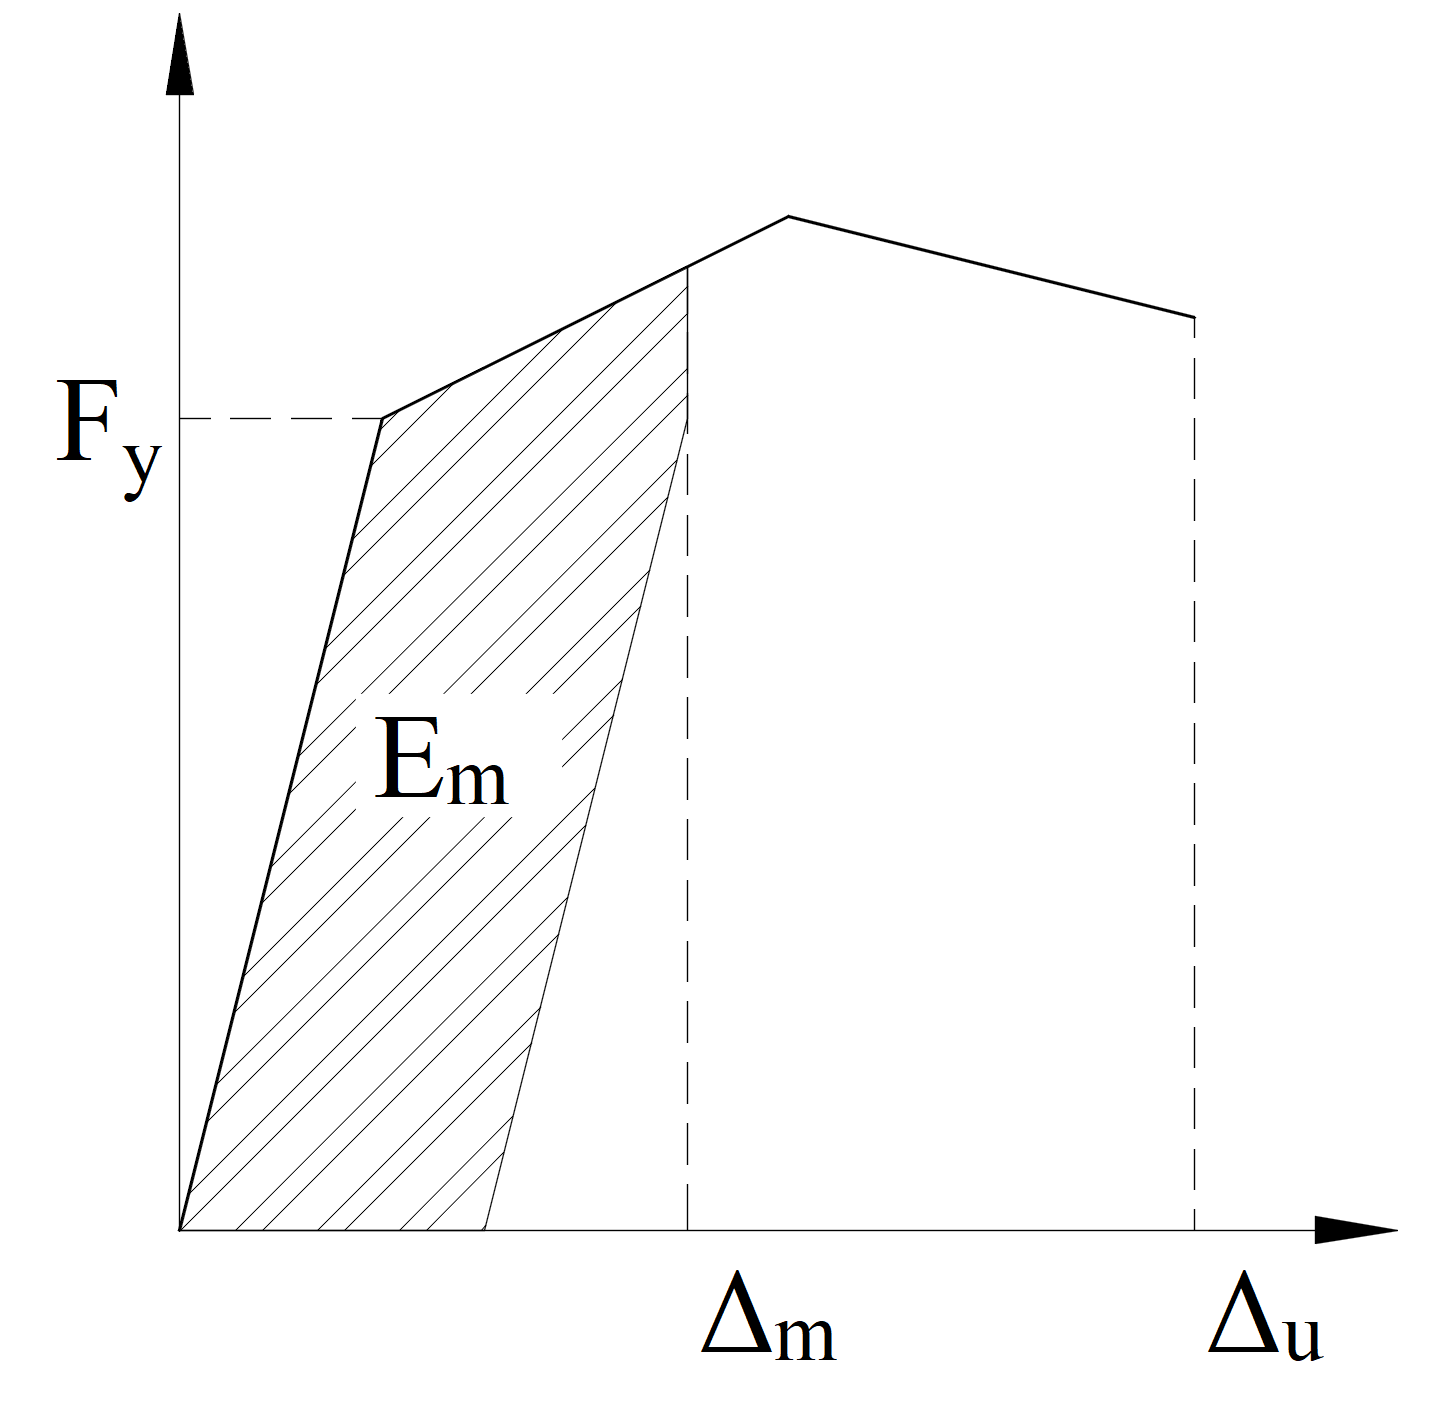
\includegraphics[width=0.50\textwidth]{Chapter-2/figs/Park_and_Ang_Model}
\caption{Park and Ang conceptual scheme}
\label{fig:Paa}
\end{figure}

Equation \ref{eq.DamageIndex} was derived for concrete elements. The first term here is a simple, pseudo-static displacement measure. The second term accounts for cumulative damage. This concept is shown in \fref{fig:Paa}. The advantages of this model are its simplicity and flexibility in adapting the model to correlate with experimental data. After calculating the damage index, this can be classified according to the damage index level defined by Park and Ang \cite{Young-JiPark1985}. The damage index level classification is shown in Table \ref{tab:DI_Level}.
\begin{table}[htbp]
    \caption{Damage index level classification \cite{Young-JiPark1985}}
	\label{tab:DI_Level}
	\centering	
        \begin{tabular}{lll}
        \hline
        Level & Damage index (DI)               & Damage measure                                             \\ \hline
        I     & DI\textless{}0.1                & No damage; localized minor cracking                        \\
        II    & 0.1\textless{}DI\textless{}0.25 & Minor damage; light cracking throughout                    \\
        III   & 0.25\textless{}DI\textless{}0.4 & Moderate damage; severe cracking; localized spalling       \\
        IV    & 0.4\textless{}DI\textless{}1.0  & Severe damage; crushing of concrete; reinforcement exposed \\
        V     & D\textgreater{}1.0              & Loss of elemental load resistance                          \\ \hline
\end{tabular}
\end{table}

However, this model has several limitations. Firstly, the calibration of the $\beta$ coefficient with observed damage has proven to be very low ($\beta=0.05-0.15$) \cite{Young-JiPark1985} \cite{Ghosh2015}, rendering the second term relatively inconsequential compared to the contribution of the first term. A sample result is taken from Gosh et al \cite{Ghosh2015}, which applied a modified version of the Park and Ang damage index in terms of the moment ($M_{y}$), the rotation ($\theta_y$), and curvature ductility ($\mu$). The modified model is expressed in \eref{eq.DamageIndexGhosh}.

\begin{equation}
	D=\frac{\mu_{m}}{\mu_{u}}-\beta\frac{E_h}{M_{y}\theta_y\mu{u}}
	\label{eq.DamageIndexGhosh}
\end{equation}

Using the following values: $\mu_{m}=4.93$; $\mu_{u}=17.02$; $M_{y}=8751.375$; $\theta_y=0.0042$; $E_{h}=119.07$; $\beta=0.05$ 

And substituting in equation \eref{eq.DamageIndexGhosh}:
\[
 D=\frac{\mu_{m}}{\mu_{u}}-\beta\frac{E_h}{M_{y}\theta_y\mu{u}}=0.3
	\]
\textbf{First term}:
\[
\frac{\mu_{m}}{\mu_{u}}=\frac{4.93}{17.02}=0.2897
\]
\textbf{Second term}: 
\[	
	\beta \frac{E_h}{M_{y}\theta_y\mu{u}}=0.05\frac{119.07}{8751.375*0.0042*17.02}=0.0103
\]

It can be seen that 97\% of the damage index comes from the first term, which is the elastic term, and the inelastic part is only 3\% of the total. 

Despite its limitations, several studies have used or modified this model to study the effects of cumulative damage for different structures. Those of relevant importance are those performed by Kunnath et al \cite{Kunnath1992}, who used a modified Park and Ang model, to account for damage at the local level for elements in the structural analysis program IDARC 3.0. In this software, for the case of multiple degrees of freedom buildings they also added parameters to consider the damage at the inter-story level and the global model. Ghosh et al \cite{Ghosh2015} developed a damage accumulation framework to estimate the probability of exceeding a damage index for multiple ground motions. Other regressions have been proposed \cite{Khashaee}, \cite{Fajfar1992}, \cite{Roufaiel} but show no improvement in assessing the damage state of a structure. While these studies provide an insight into some of the characteristics of damage accumulation they, still rely on the Park and Ang model and therefore carry the same limitations.

Krawinkler (1987) \cite{Krawinkler1987} proposed a method that considered damage as a function of low cycle fatigue parameters. The form of the Krawinkler damage index for steel components, weldments, and local buckling has a general shape of the Miner model. This model relies on the accumulation of plastic deformations. While this model has proven to work well for the evaluation of individual steel structure elements, it does not provide a way to generalize damage for other types of structures.


\section{Multiple earthquake loading}

The evaluation of multiple seismic events has been scarcely studied; however, their effects have been felt in numerous earthquake sequences such as the Christchurch 2010, Umbria-Marche Earthquake 1997 and the Puerto Rico Earthquakes 2020. The hypothesis is that accumulation of damage will restart in a smaller seismic event to achieve a prescribed limit state, similar to how corrosion and other aging phenomena might impact the intensity needed to achieve a future limit state. 

In the literature the study of multiple earthquake loading can be classified in two groups:

\begin{itemize}
	\item Mainshock-aftershock sequences
	\item Mainshock sequences
\end{itemize}

These studies have shown what are some of the effects of multiple earthquake loading for different structures.

\subsection{Mainshock-aftershock sequences loading }

Strong aftershocks can increase the state of damage of a building or even collapse an already damaged structure. It is therefore important to quantify the increase of seismic demands in structures due to aftershock loading. In recent years different studies have been carried out to develop methodologies that consider these effects.

Tesfamariam et al \cite{Tesfamariam2015} investigated the increase in the demands for multiple degrees of freedom systems (MDOF). They conducted a parametric study of RC bare frame buildings and RC frame with infill masonry buildings. The main parameter of study focused on the thickness of the infill frames ranging from 75mm - 125 mm. In addition, a series of mainshock-aftershock sequences were applied, selected for the area of Vancouver, BC. The mainshock-aftershock sequence were selected using the conditional mean spectra (CMS) over the period range of the structures. The motions considered in their study were different for the bare frame and the infill frames. The bare frame was subjected to a mainshock  followed by three aftershocks, while those of the infill frame consisted of on mainshock followed by one aftershock each. Their results showed that there is an increase of 10\% in the inter-story drift demands for the RC bare frame structures. For the case of infill frames the inter-story drift did not significantly increased. Their study used FEMA 356 \cite{FEMA2000} to define the performance limit states. FEMA 356 drift performance limit states are based on linear regression on observed damage to drift level obtained from experimental tests. The linear regression compared to the experimental results have high dispersion. Therefore, it is possible that in the study by Tesfamariam et al, that while a drift limit state did not increase after applying a MS-AS sequence, a higher strain was reached in some of the components due to the MS-AS sequence, and as consequence a higher strain performance limit state could have been reached. Thus emphasizing the importance of using strain performance limit states. Similarly, Raghunandan et al \cite{Raghunandan2015} studied the vulnerability of RC frame structures. Their study showed that depending on the level of interstory drift achieved during the mainshock the additional damage experienced during the aftershock will be different. For example, the authors showed that for an RC frame that experiences 4\% or more interstory drift in the mainshock, the median capacity to resist aftershock shaking is reduced by about 40\%. Furthermore, other studies have focused on the behavior of single degree of freedom (SDOF) systems response to mainshock-aftershock (MS-AS) sequences \cite{Hatzigeorgiou2009}\cite{Manafpour2019}. Hatzigeorgiou et al focused on determining the inelastic displacement coefficient variation due to the MS-AS sequence. Their study concluded that there is an increase in the inelastic displacement demands, however, the limitations in their study did not report what happens to the performance limit states. Further, Manafpour et al studied the seismic drift behavior of structures to MS-AS sequences for far-field earthquakes and near-field earthquakes. Their study concluded that for SDOF structures near-field earthquake sequences were the most damaging, increasing the drifts by as much as 45\% compared to a structure subjected to the main shock only.

Researchers have applied two earthquake selection procedures for mainshock-aftershock sequences. The first method, incremental dynamic analysis (IDA), consists of 1)subjecting the nonlinear building model to a ground motion having a particular intensity, 2) recording the response of the structure \cite{Vamvatsikos2002}, 3)in successive analyses, the ground motion is incrementally scaled to a higher intensity measure (IM), and 4)the structural response is recorded in each analysis. The IDA procedure was extrapolated to for MS-AS sequence as follows: 1)Apply the IDA to the mainshocks to obtain 11 drift damage levels raging from 0.5\% to 5.5\% of interstory drift in the structure, 2) after each mainshock include an incrementally scaled aftershock with a 4 seconds gap between the mainshock and the aftershock, and 3)Change the polarity of the aftershock, which refers to the direction of the aftershock variation to the mainshock. \fref{fig:MS-AS_Luco} shows one of the resulting MS-AS sequences using the IDA methodology. Due to the use of scaling factors the IDA methodology uses artificial mainshock-aftershock sequences. In addition, the IDA analysis can be computationally expensive. For instance, the authors reported a total of 9900 ground motion sequences per structure.

\begin{figure}[htbp]
\centering
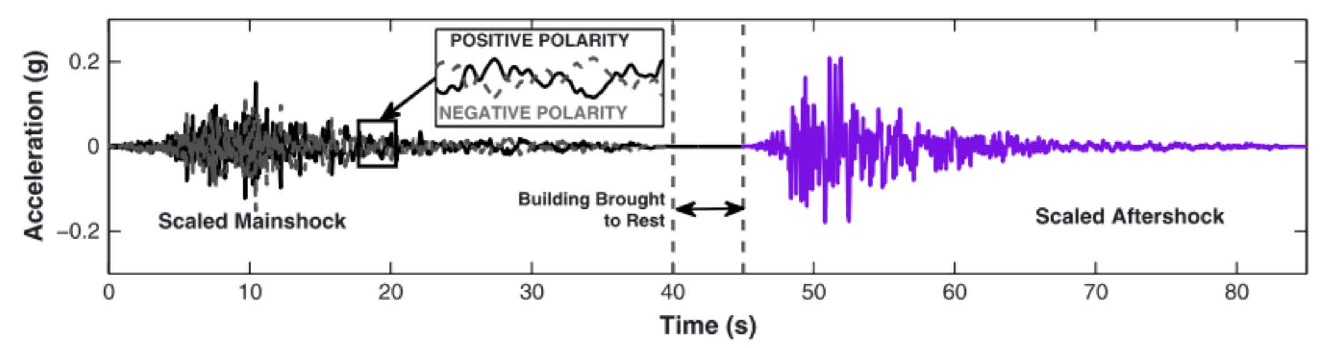
\includegraphics[width=0.6\textwidth]{Chapter-2/figs/MS-AS_sequence_Luco}
\caption{Mainshock-aftershock sequence train of ground motions \cite{Raghunandan2015}}
\label{fig:MS-AS_Luco}
\end{figure}

The second method consists of matching the MS-AS sequences to a site seismic hazard curve obtained from a probabilistic seismic hazard analysis (PSHA). Tesfamariam \cite{Tesfamariam2015} used conditional mean spectra (CMS) to match and select mainshock-aftershock sequences for structures located in Vancouver, BC. Their study selected MS-AS sequences from two databases of ground motions, NGA-West2 \citep{Ancheta2014}, and the K-NET//KiK-net \cite{NIEDK-NETKiK-net2019}. The CMS process consists of computing the expected response spectrum associated with a target spectral acceleration ($Sa$) value at a single period, using the known values from the PSHA such as the magnitude, distance, and $\epsilon$ values. In their study the authors used CMS to select the MS-AS sequences for different earthquake scenarios a)Crustal earthquake, b) Interface, and c) Inslab. They hypothesized that different earthquake scenarios would have different MS-AS sequence characteristics such as higher spectral acceleration ($Sa$) values at short periods for interface earthquakes, and high $Sa$ values at longer periods for crustal earthquakes.They argue that using the CMS method makes the selection of ground motion consistent with the seismological features of the area of study. \fref{fig:MS-AS_Goda} shows this selection for a structure with a 0.4s period for crustal earthquakes. The CMS method adapts to the site conditions, no scaling of MS-AS is required since the selection is optimized to ground motion sequences stored in the databases. Since the CMS method uses site-specific data, it can be a part of an analytical framework that can be adapted to different seismic regions.
\begin{figure}[htbp]
\centering
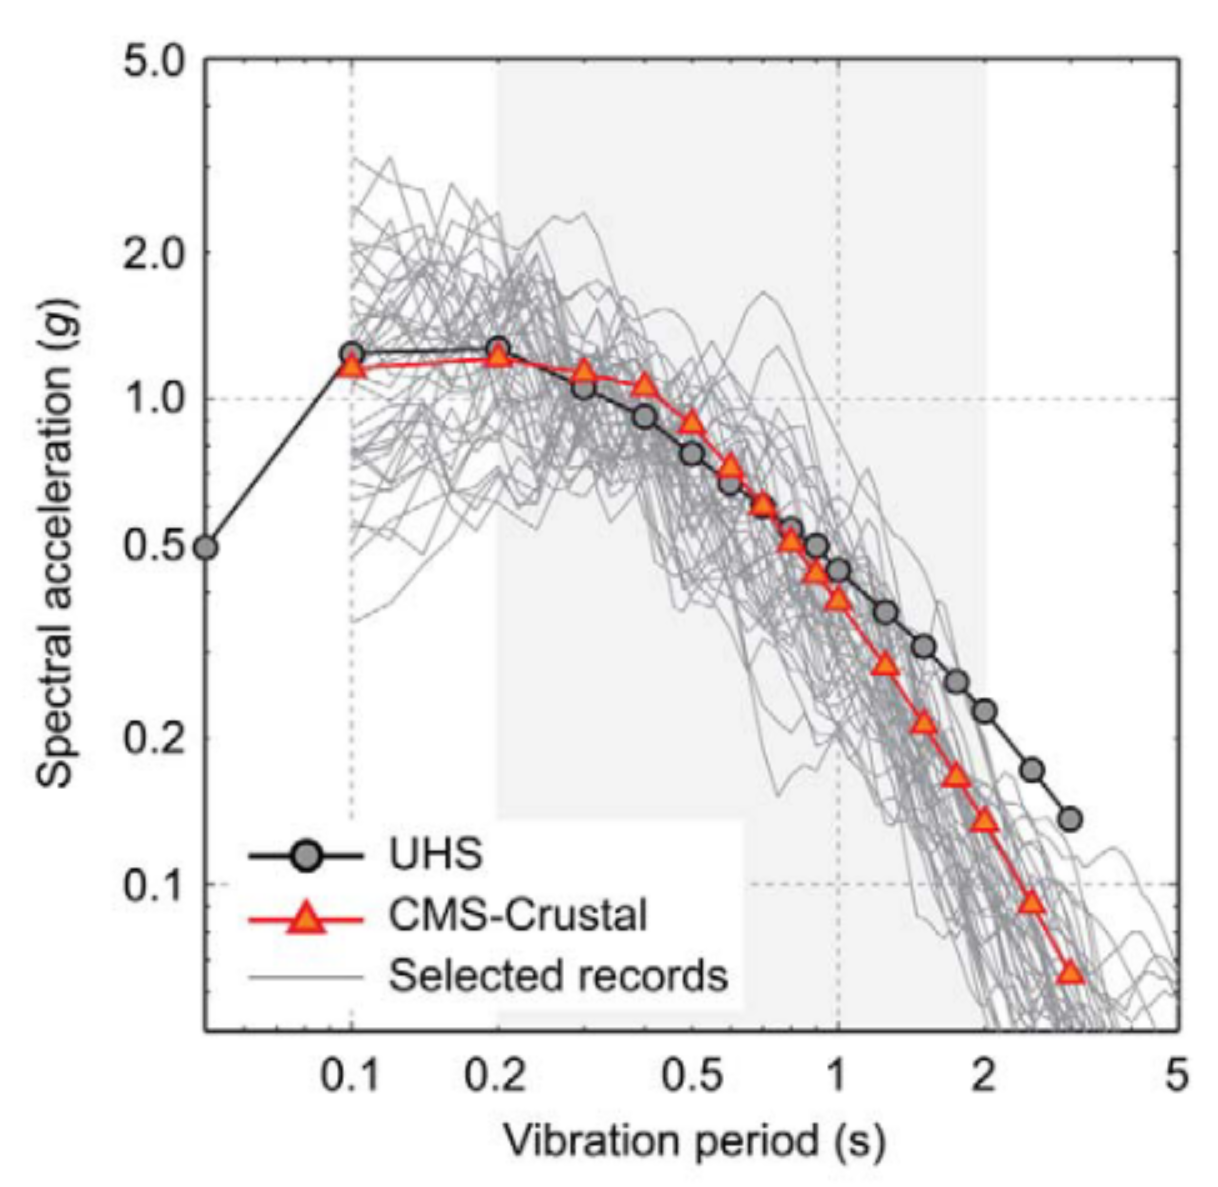
\includegraphics[width=0.5\textwidth]{Chapter-2/figs/CMS-Tesfamariam_MS-AS_seq}
\caption{Mainshock-aftershock sequence selection at T=0.4s for crustal earthquakes in Vancouver, British Columbia \cite{Tesfamariam2015}}
\label{fig:MS-AS_Goda}
\end{figure}

\subsection{Mainshock sequences loading}

Reliable temporal prediction of earthquakes is currently impossible.  However, for a large region, earthquakes recurrence time can be modeled reasonably well as a Poisson process. Sunasaka \cite{Sunasaka1993} developed mainshock sequences that followed a Poisson process. Their study focused on the accumulation of damage due to mainshock sequences, and mainshocks-aftershocks sequences. Damage accumulation was accounted for by the Park and Ang index. The authors used ground motion prediction equations to develop artificial mainshock sequences. Their study calculated the recurrence period, magnitude, location and peak ground acceleration for each of the mainshocks. The author subjected an SDOF bridge in Eureka, CA to the mainshock sequence shown in   \fref{fig:MS-MS_Sunasaka}. While the results shows a significant increase in the damage index due to mainshock sequences, the conclusions are limited by the assumption that a Poisson process can be applied to single faults, which has not shown good correlation with observed events\cite{Shearer2009}. While this study shows what could be possible if mainshocks were predictable in small regions, more advances in seismology are needed to confidently apply the proposed methodology.

\begin{figure}[htbp]
\centering
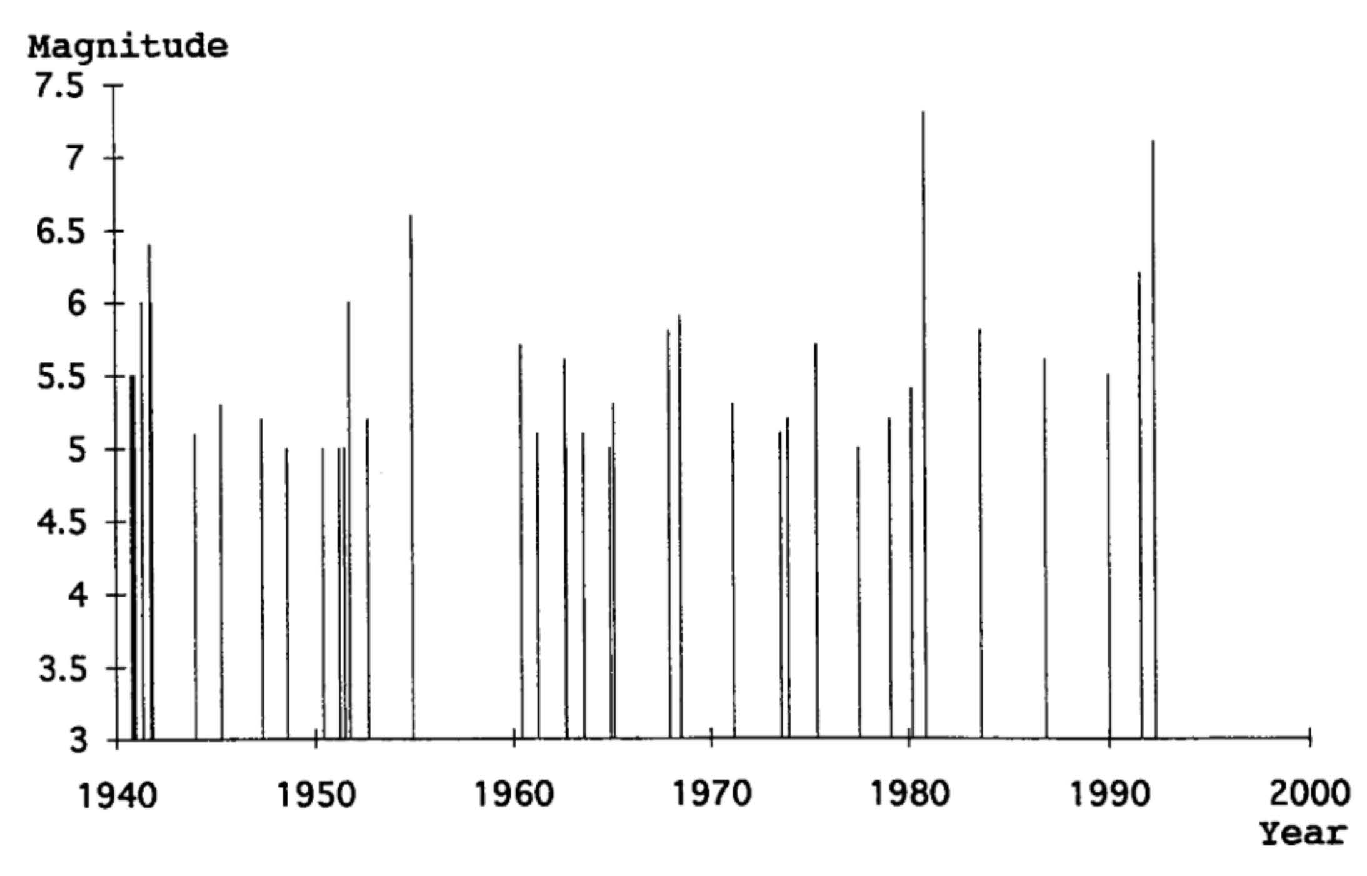
\includegraphics[width=0.5\textwidth]{Chapter-2/figs/Mainshock_sequence_01}
\caption{Mainshock sequence selection at Eureka, CA \cite{Sunasaka1993}}
\label{fig:MS-MS_Sunasaka}
\end{figure}

Other studies have used three equally spaced mainshocks \cite{Hatzigeorgiou2009}. The three equally spaced mainshocks can be deployed without much computational effort, however, there is not a seismological basis for the use of three equally spaced mainshocks. Therefore, the use of this methodology would be limited to a scenario analysis and not useful for analysis and design, since the probabilities of three equally spaced in time mainshocks on any given structure is very low.

\section{Aging of structures}

There have been attempts by many researchers to characterize the aging of structures.

In recent years studies have focused on the effect of cumulative damage. These studies have focused on assessing the damage accumulation considering multiple earthquakes, corrosion and service life of the structure. Two field of study have been observed:

\begin{itemize}
	\item Probabilistic framework
	\item Fragility curves
\end{itemize}

\textbf{Probabilistic Framework}

One of the most widely used probabilistic frameworks is the Pacific Earthquake Engineering Research Center (PEER) Performance Based Design (PBD). PEER PBD can be expressed by the following equation:
\begin{equation}
\nu_{DM}(dm^{LS})=\iint D_{DM|EDP}(dm|edp)|,dG_{EDP|IM}(edp|im)||\,d\nu_{IM}(im)|
\end{equation}

Mackie et al \cite{Mackie2007} using  the PEER PBD, developed the performance based damage design (PBDD) and performance based loss design (PBLD) by defining the probabilistic demand, damage, and loss model parameters in terms of reinforced concrete column damage. The RC column damage was defined in terms of mean drift ratios obtained from the PEER structural performance database (http://nisee.berkeley.edu/spd/). The drift limit states considered in their study were concrete spalling, bar buckling and failure. In their study, failure was defined as the first occurrence of the database fields for reinforcing bar fracture and loss of axial load-carrying capacity 

The authors show that for a given intensity measure ($IM$) and a confidence level of achieving a limit state, it is possible to then define the probability  of exceeding that limit state. The authors used peak ground velocity ($PGV$) as their intensity measure. While this methodology was able to define damage and incorporate it into the PEER PBD framework, the authors did not consider strain to define the limit states. In a PEER report Mackie et al studied seismic demands for performance-based design of bridges. In the report they performed a design parameter sensitivy analysis in which they evaluate different intenisity measures. Their analysis showed that the optimal $IM$ to predict most engineering demand parameters ($EDP$) is the first mode spectral displacement $Sd(T_{1})$  \cite{Mackie2003}. However, at the time their report was written the $Sd(T_{1})$ did not show good correlation with strain as the $EDP$, and as a consequence they did not recommended to use strain as a predictor of structural performance. Nonetheless, a recent study presented by Krish et al shown that  new advancements in the modeling of plastic hinge forming members can more accurately relate strain and $S_{d}(T_{1})$. They conclude that the use of these parameters is well suited to predict the performance of structures \cite{Krish2018}.

\textbf{Fragility Curves}

Another common trend in this subject is the use of fragility curves to estimate the effect of damage in structures. Two main approaches were found in the literature. One of them relied on the Park and Ang Model damage index to define damage, while the second approach related damage to drift.

Ghosh et al \cite{Ghosh2015} formulated a damage accumulation framework. Their study relied on the Park and Ang Damage index explained in the previous section. The study performed a series of nonlinear time history analyses for two cases:

\begin{itemize}
	\item Using a constant main shock hazard occurrence rate (3 main shocks in a 50-year period)
	\item Mainshock - Aftershock series using a time-dependent aftershock hazard occurrence rate
\end{itemize}

The results from their study showed regression equations that statistically predict the damage index as a function of earthquake intensity and damage history. This study revealed that for both mainshock and aftershock scenarios there was a significant increase in the probability of damage index exceeding a damage index level (as defined in Table \ref{tab:DI_Level}) under repeated shock scenarios. While this study shows the importance of considering damage accumulation, these results have to be taken with caution, since they present the same disadvantages as the Park and Ang damage index.

Ghosh et al \cite{Ghosh2010} also studied the effects of corrosion on time dependent seismic fragility curves. Their study characterizes corrosion in concrete columns as a continuous phenomenon that occurs as a function of time. The authors also considered the effects of corrosion on steel bridge bearings. The authors then ran a series of NLTHA analyses for different aging times of the structures. Based on their analysis, time dependent fragility curves were presented. The results showed that as time increases, and corrosion increases as a consequence, the probability of exceeding a limit state increases. In their study, limit states were defined on the basis of inter-story drifts which were obtained from experimental results and field observations \cite{Padgett2007}. It is important to mention that the limit states used in their study were not defined on the basis of strains or other structural property. Instead the limit states came from a survey performed in central and southeastern United States departments of transportation, on the premise of a range of experienced inter-story drifts and the time taken to repair them. In addition, assuming that corrosion is a continuous process has to be cautiously taken as valid. This is because site information such as temperature, water to cement ratio, the addition of cementitious materials such as silica fume, and the environment (e.g. coastal vs inland) affect the rate of propagation of corrosion\cite{Thoft-Christensen}.

While these studies provide a general view on how damage increases the likelihood of observing collapse or deterioration of the seismic performance, the methods used to arrive at those conclusions can be misleading since the definition of damage as either a Damage Index or Drift are not the best parameters to quantify the damage. It is our belief that strain-based limit states will provide a better understanding of the implications of damage accumulation.

\section{Research Gap}

Many studies have tried to show the importance of quantifying the effects of accumulated damage and multiple shocks throughout the lifetime of a structure.  Therefore, it is important to develop a model that establishes the likelihood of achieving a limit state as the structure ages. In addition,  it is important to understand the impacts of aging on bridge seismic performance. Furthermore, bridges in seismic areas can be subjected to main shock and aftershocks. Therefore, a methodology that incorporates both aging and multiple seismic events is needed.

Damage accumulation is a topic that has been gaining momentum in the engineering community, this study will better inform  the potential future conditions of a structure to stakeholders such as state DOTs, building owners, and practicing engineers. In the literature it was observed that damage accumulation has been studied using the Park and Ang damage index or drift-based limit states to measure damage accumulation. Different researchers have also included corrosion into their scope of analysis, which shows that aging conditions play an important role in the deterioration of a structure. In addition, Krish \cite{Krish2018} determined that spectral displacement at first effective period is an improved intensity measure (IM), while the past literature used the peak ground acceleration (PGA) as the controlling IM. This research will develop a parametric study using a series of single degree of freedom (SDOF) systems, subjecting them to different conditions such as corrosion, and steel strain aging. The SDOF structures will be subjected to a sweep of ground motions using nonlinear time history analysis to obtain maximum strain demands. With the results from NLTHA, fragility functions will be used to show the increase in the likelihood of reaching a performance limit state due to aging of the structure. In addition, this research will provide the engineering community with a design framework to account for damage accumulation in their analysis and guide decisions on the resiliency of a structure. In addition, this study will provide a methodology in which the Direct Displacement-Based Design (DDBD) is modified to consider the effects of damage and aging conditions.

\subsection{Objectives}
The main goal of this research is to provide a design methodology to consider damage for performance based seismic design of structures. In addition, this study will demonstrate the implications of aging conditions and multiple earthquakes for the design of bridge RC columns.


\begin{itemize}
	\item Incorporate different aging conditions and develop fragility curves that considers strain limit states as a measure of damage
	\item Establish limit states for corroded rebars
	\item Inform the research community of the necessary methodology to appropriately mimic real corrosion process in material experiments of corroded rebars, which can later be extrapolated to large scale testing of RC columns subjected to corrosion
	\item Consider the effects of multiple earthquakes for  two cases: (1) Mainshock-Aftershock sequence, and (2) Mainshock-Aftershock sequence with the effects of time between the mainshock and the aftershock.
	\item Incorporate these results into the Direct Displacement Based Design (DDBD) methodology, through the use of factors that correspond to the aging conditions
\end{itemize}